\chapter{Hysteretic neural networks\label{cha:chapter2}}

% section{Hysteretic neural networks\label{sec:chapter2:hnn}}
\section{Play and Prandtl-Ishlinskii networks\label{sec:chapter2:play-and-pi-networks}}

Consider $K > 0$ play operators. Each of them maps an initial state $p_{0}^{k} \in \mathbb{R} $ and an input sequence $x_1, x_2, \ldots$ to an output sequence $p_{1}^{k}, p_{2}^{k}, \ldots \ $, i.e.,

\begin{equation*}
  p_{0}^{k}, (x_1, x_2, \ldots) \mapsto (p_{1}^{k}, p_{2}^{k}, \ldots), k = 1, \ldots, K
\end{equation*}
The $k$th play operator is given by:

% \begin{equation}\label{eqn:chapter2:play-operator}
%   p_{n}^{k} = G(x_{n}, p_{n-1}^{k}, w^{k}) := p_{n-1}^{k} + \Phi(w^{k} x_{n} - p_{n-1}^{k}), n = 1, 2, \ldots, N
% \end{equation}

\begin{equation}\label{eqn:chapter2:play-operator}
  p_{n}^{k} := p_{n-1}^{k} + \Phi(w^{k} x_{n} - p_{n-1}^{k}), n = 1, 2, \ldots, N
\end{equation}

where $w^{k}$ are parameters and

\begin{equation}\label{eqn:chapter2:phi}
  \begin{aligned}
    \Phi(x) =
    \begin{cases}
      x - 0.5, & x > 0.5 \\
      0,               & -0.5 \le x \le 0.5 \\
      x + 0.5, & x < 0.5
    \end{cases}
  \end{aligned}
\end{equation}

See \myfigref{fig:chapter2:phi}

\begin{figure}[htb]
    \centering
    \subfloat[$\Phi(x)$]{
        \documentclass{standalone}
\usepackage{pgfplots}
\pgfplotsset{compat=1.11}
\begin{document}
% Place the TikZ picture in a figure environment.
%\begin{figure}[htb]
% h: here, t: top, b: bottom, p: page of float
%% https://tex.stackexchange.com/questions/39017/how-to-influence-the-position-of-float-environments-like-figure-and-table-in-lat
%% ! indicates that some restrictions should be ignored (discussed later)
%% h indicates that the float is allowed to be placed inline
%% t indicates that the float is allowed to go into a top area
%% b indicates that the float is allowed to go into a bottom area
%% p indicates the the float is allowed to go on a float page or column area

    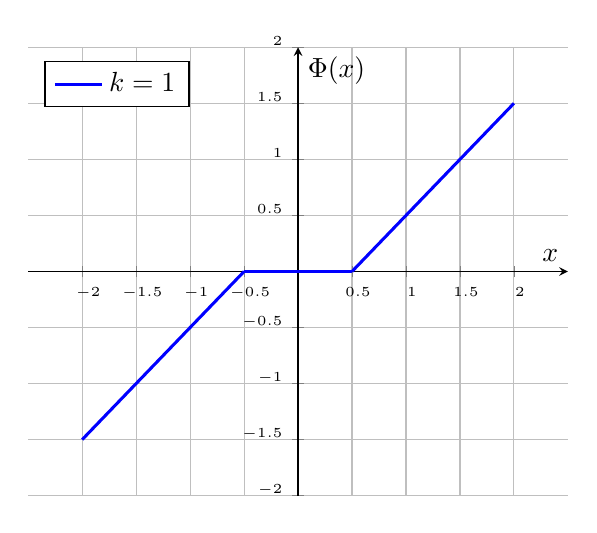
\begin{tikzpicture}
        \begin{axis} [
            xmin=-2.5, xmax=2.5, ymin=-2, ymax=2, grid=both,
            ylabel={$\Phi(x)$}, xlabel={$x$},
            xtick={-2,-1.5,...,2}, ytick={-2,-1.5,...,2},
            xticklabel style={font=\tiny, xshift=0.5ex},
            yticklabel style={font=\tiny, yshift=0.5ex},
            axis line style={->},
            axis x line=middle,
            axis y line=middle,
            legend pos=north west,
        ]
        \addplot+[mark=none, line width=1.1, color=blue, domain=-2:-0.5] {x+0.5};
        \addplot+[mark=none, line width=1.1, color=blue, domain=-0.5:0.5] {0};
        \addplot+[mark=none, line width=1.1, color=blue, domain=0.5:2] {x-0.5};
        \addlegendentry{$k=1$}
        \end{axis}
    \end{tikzpicture}

\end{document}
        \label{fig:chapter2:phi}
    }
    \subfloat[$\text{Play(x)}$]{
        \input{./tikz/play-by-phi}
        \label{fig:chapter2:play-by-phi}
    }
    \caption{hello}
\end{figure}

It can be represented as a recurrent neural network, see Fig. \ref{fig:chapter2:phi}. Note that in such a form the network is not feed-forward.
One can unfold it to make it feed-forward, see Fig. \ref{fig:chapter2:play-operator}

\begin{definition}
We call this network a \textsl{play network}. If there are \textsl{m} elements in the sequence ${x_n}$, we say the unfolded network is \textsl{m-unfolded}
\end{definition}

For example, the network in Fig. \ref{fig:chapter2:unfolded-nn} is 2-unfolded.



\section{Training a PI network\label{sec:chapter2:training-pi-network}}
Assume we are given an input sequence $x_1, x_2, \ldots, x_N$ and an output sequence $q_1, q_2, \ldots, q_N$. We perform the following steps in cycle until convergence.

\begin{enumerate}
\item Preparing initial states for the $m$-unfolded network: Fix a vector of initial states $P_0$ and all the weights (denoted by $W$). For each $k=1, \ldots, K$, we calculate recursively $p_{1}^{k}, p_{2}^{k}, \ldots, p_{N}^{k}$ by formula \ref{eqn:chapter2:play-operator}. We denote the corresponding (intermediate) states of the \textbf{PI} operator by
  \begin{equation*}
    P_n = (p_{n}^{1}, \ldots, p_{n}^{K}), n = 1, \ldots, N.
  \end{equation*}
\item Preparing inputs for the $m$-unfolded network: We fix $m$ and group the input sequence into $m$-tuples:
  \begin{equation*}
    \mathbf{x_1} := (x_1, \ldots, x_m), \quad \mathbf{x_2} := (x_2, \ldots, x_{m+1}), \quad \ldots,
  \end{equation*}
  which gives $M := N-m$ tuples $\mathbf{x_1}, \ldots, \mathbf{x_M}$. Next we form a new set of inputs for the $m$-unfolded network, attaching the vectors of intermediate states:
  \begin{equation*}
    \mathbf{y_1} := (P_0, \mathbf{x_1}), \quad \mathbf{y_2} := (P_1, \mathbf{x_2}), \quad \ldots,
  \end{equation*}

\item Training the $m$-unfolded network: We train by stochastic gradient descent the feed-forward $m$-unfolded \textbf{PI} network
  \begin{equation*}
    \mathbb{R}^{K} \times \mathbb{R}^{m} \ni \mathbf{y} \mapsto F_{m}(\mathbf{y}) \in \mathbb{R}^m
  \end{equation*}
  with the inputs $\mathbf{y_1}, \ldots, \mathbf{y_M}$ and the true targets $\mathbf{q_1}, \ldots, \mathbf{q_M}$, where
  \begin{equation*}
    \begin{aligned}
      \mathbf{q_1} = (q_1, \ldots, q_m), \quad 
      \mathbf{q_2} = (q_2,\ldots, q_{m+1}), \quad 
      \ldots
    \end{aligned}
  \end{equation*}

% \item We update the initial state $P_0$:
%   \begin{equation*}
%     P_{0}^{new} := P_{0} - \nabla_{P_0} (F_m(P_0, \mathbf{x_1}) - \mathbf{q_1})^2
%   \end{equation*}
\item Updating weights $W$ and initial state $P_0$ 
  \begin{eqnarray*}
    W^{new} := W - \nabla_{W} (F_m(P_0, \mathbf{x_1}) - \mathbf{q_1})^2 \\
    % P_{0}^{new} := P_{0} - \nabla_{P_0}(F_m(P_0, \mathbf{x_1}) - \mathbf{q_1})^2
  \end{eqnarray*}
% \item \mytodo{TODO: Training state}
% \item \todo{TODO: Training weights}

\end{enumerate}

% \subsection{Analysis of $p_0$}
% For $k>0$
% \begin{equation}
%   \begin{aligned}
%     \Phi(x) =
%     \begin{cases}
%       k(x - \frac{1}{2}), & x \in [\frac{1}{2}, +\infty) \\
%       0,               &  x \in (-\frac{1}{2}, \frac{1}{2}) \\
%       k(x + \frac{1}{2}), & x \in (-\infty, \frac{1}{2}]
%     \end{cases}
%   \end{aligned}
% \end{equation}

% \begin{eqnarray*}
% p_n &=& \Phi(w x_{n} - p_{n-1})- p_{n-1} \\
% \frac{\partial p_{n}}{\partial p_{n-1}} &=& 1- \frac{\partial \Phi(u_n)}{\partial u_n}\Bigr|_{\substack{u_n=w x_{n} - p_{n-1}}} 
% \end{eqnarray*}

% \begin{equation}\label{eqn:chapter2:derviation-phi}
%   \begin{aligned}
%     \frac{\partial \Phi(u_i)}{\partial u_i} =
%     \begin{cases}
%       k, & p_{n-1} \in (-\infty, w x_{n}-\frac{1}{2}] \cup [w x_{n}+\frac{1}{2}, +\infty) \\
%       0, &  p_{n-1} \in (w x_{n}-\frac{1}{2}, w x_{n}+\frac{1}{2})
%     \end{cases}
%   \end{aligned}
% \end{equation}

% \begin{equation}\label{eqn:chapter2:dynamic-p0}
% \frac{\partial p_{n}}{\partial p_0}= \prod_{i=1}^{n} \frac{\partial p_{i}}{\partial p_{i-1}} = \prod_{i=1}^{n} \left(1- \frac{\partial \Phi(u_i)}{\partial u_i}\Bigr|_{\substack{u_i=w x_{i} - p_{i-1}}}\right)
% \end{equation}


% Combining \ref{eqn:chapter2:derviation-phi} and \ref{eqn:chapter2:dynamic-p0}, if $n$ is sufficiently large, we conclude that 
% \begin{enumerate}
%     \item $k \in (0, 2]$, gradient on $p_0$ vanishes
%     \item $k \in (2, +\infty)$, gradient on $p_0$ explodes.
% \end{enumerate}

% Solution: using batch training method may avoid gradient vanishing and exploding, however, the batch size cannot be too large. 